\newpage
\solutions{Kombinatoryka z elementami geometrii}

\begin{problem}{1}
	Każdemu punktowi $A$ na płaszczyźnie przyporządkowano pewną liczbę rzeczywistą $f(A).$ Wiadomo, że $f(M) = f(A) + f(B) + f(C),$ gdy $M$ jest środkiem masy trójkąta $ABC.$ Wykazać, że $f(A) = 0$ dla wszystkich punktów $A.$
\end{problem}

\begin{center}
	\begin{tikzpicture}
		\tkzDefPoint(0,0){A}
		\tkzDefPoint(2,0){B}
		\tkzDefTriangle[equilateral](A,B) \tkzGetPoint{C}
		\tkzDefMidPoint(A,B) \tkzGetPoint{M}
		\tkzDefMidPoint(B,C) \tkzGetPoint{K}
		\tkzDefMidPoint(A,C) \tkzGetPoint{L}

		\tkzCentroid(A,B,C) \tkzGetPoint{O}
		\tkzCentroid(A,L,M) \tkzGetPoint{O_1}
		\tkzCentroid(B,K,M) \tkzGetPoint{O_2}
		\tkzCentroid(C,K,L) \tkzGetPoint{O_3}

		\tkzDrawPoints(A,B,C,K,L,M,O,O_1,O_2,O_3)
		\tkzDrawSegments(A,B B,C C,A K,L L,M M,K)
		\tkzLabelPoints[below](A,M,B)
		\tkzLabelPoints[right](K)
		\tkzLabelPoints[above](C)
		\tkzLabelPoints[left](L)
	\end{tikzpicture}
\end{center}

\noindent
Rozpatrzmy dowolny trójkąt równoboczny $ABC$. Niech $K$, $L$ i $M$ to będą środki odpowiednio $BC$, $AC$ i $AB$. Niech $O$ będzie środkiem ciężkości trójkąta $ABC$, a punkty $O_1$, $O_2$ i $O_3$ środkami ciężkości trójkątów $ALM$, $BKM$ i $CKL$ odpowiednio. Z założeń zadania mamy
\begin{align*}
	f(O_1) &= f(A) + f(L) + f(M), \\
	f(O_2) &= f(B) + f(M) + f(K), \\
	f(O_3) &= f(C) + f(K) + f(L).
\end{align*}
Dodając powyższe równości stronami otrzymujemy
\[
	f(O_1) + f(O_2) + f(O_3) = (f(A) + f(B) + f(C)) + 2(f(K) + f(L) + f(M)). \quad (*)
\]
Zauważmy, że punkt $O$ jest środkiem ciężkości trójkątów $ABC$ i $O_1O_2O_3$, stąd
\begin{align*}
	f(O) &= f(A) + f(B) + f(C), \\
	f(O) &= f(O_1) + f(O_2) + f(O_3),
\end{align*}
czyli
\[
	f(O_1) + f(O_2) + f(O_3) = f(A) + f(B) + f(C). \quad (**)
\]
Łącząc równości $(*)$ i $(**)$ otrzymujemy, że
\[
	f(K) + f(L) + f(M) = 0.
\]
Pozostaje zauważyć, że punkt $O$ jest środkiem masy trójkąta $KLM$, skąd
\[
	f(O) = f(K) + f(L) + f(M) = 0.
\]
Zauważmy, że dla dowolnego punktu na płaszczyźnie można wybrać taki trójkąt równoboczny, aby ten punkt był środkiem jego boku. Toteż dla każdego punktu $X$ mamy $f(X) = 0$.


\begin{problem}{2}
	Dana jest liczba $n \geqslant 3$ oraz pewne $n$ par liczb rzeczywistych  $(x_1,\; y_1)$, $(x_2,\; y_2)$, ..., $(x_n, \; y_n)$, że dla każdej liczby całkowitej $1 \leqslant i \leqslant n$ zachodzi
	\[
		x_i^2 + y_i^2 = 1.
	\]
	Wykazać, że istnieją takie liczby $i$ oraz $j$, że zachodzi nierówność
	\[
		(x_i - x_{j})^2 + (y_i - y_{j})^2 \leqslant \frac{4\pi^2}{n^2},
	\]
	przy czym $x_{n + 1} = x_1$ oraz $y_{n + 1} = y_1$.
\end{problem}

\noindent
Rozpatrzmy punkty $A_1$, $A_2$, ..., $A_n$ na płaszczyźnie kartezjańskiej, przy czym 
\[
	A_i = (x_i, \; y_i).
\]
Zauważmy, że punkty te leżą na okręgu o środku w punkcie $(0,\; 0)$ i promieniu $1$. Chcemy wykazać, że dla pewnych $i$ oraz $j$ zachodzi nierówność
\[
	(A_iA_{j})^2 = (x_i - x_j)^2 + (y_i - y_j)^2 \leqslant \frac{4\pi^2}{n^2},
\]
czyli równoważnie
\[
	A_iA_{j} \leqslant \frac{2\pi}{n}.
\]

\begin{center}
	\begin{tikzpicture}[scale=0.7]
		\tikzset{vertex/.style = {shape=circle,draw, inner sep = 1pt, fill=black}}

		\tkzDefPoint(0,0){O}
		\tkzDefPoint(0,2){A}
		\tkzDrawCircle(O,A)
		\tkzDefPoint(1.96, 0.31){X}
		\tkzDefPoint(0.7, 1.87){Y}
		\tkzDefPoint(-0.7, 1.87){P}
		\tkzDefPoint(-2, 0){Q}
		\tkzDefPoint(-0.7, -1.87){R}

		\tkzDrawPoints(X, Y, P, Q, R)
		\tkzLabelPoint[below right](X){$A_i$}
		\tkzLabelPoint[above](Y){$A_{i + 1}$}
		\tkzDrawSegments(X,Y Y,P P,Q Q,R R,X)
		
	\end{tikzpicture}
\end{center}

\noindent
Załóżmy bez straty ogólności, że punkty leża na danym okręgu w takiej kolejności, w jakiej są one ponumerowane.

\vspace{10px}
\noindent
Zauważmy, że skoro każdy odcinek $A_iA_{i + 1}$ jest krótszy od odpowiadającego mu łukowi, to suma
\[
	A_1A_2 + A_2A_3 + ... + A_nA_1
\]
jest nie większa niż obwód danego okręgu, który wynosi $2\pi$. Stąd wynika, że pewnien z~$n$~składników tej sumy jest nie większy niż $\frac{2\pi}{n}$.

\begin{problem}{3}
	Rozstrzygnąć, czy istnieje taki wielokąt wypukły, że dla każdego jego boku i każdego jego wierzchołka, przy czym rozpatrywany wierzchołek nie należy do rozpatrywanego boku, rzut prostokątny tego wierzchołka na prostą zawierającą ten bok leży poza rozpatrywanym bokiem.
\end{problem}

\answer{Taki wielokąt nie istnieje.}

\begin{center}
	\begin{tikzpicture}\tikzset{vertex/.style = {shape=circle,draw, inner sep = 1pt, fill=black}}

		\node[vertex, label=below:$A$] (A) at (0,0) {};
		\node[vertex, label=below:$B$] (B) at (4,0) {};
		\node (A_1) at (0,3.5) {};
		\node (B_1) at (4,3.5) {};
		\node[vertex] (Y_1) at (5,1) {};
		\node[vertex] (Y_2) at (5.2,1.4) {};
		\node[vertex, label=above right:$Y$] (Y) at (4.2,2.2) {};
		\node[vertex, label=above left:$X$] (X) at (-0.5,2.1) {};
		\node[vertex] (X_1) at (-1,0.3) {};

		\draw (A) -- (B) -- (Y_1) -- (Y_2) -- (Y) -- (X) -- (X_1) -- (A);
		\draw[dashed] (A) -- (A_1);
		\draw[dashed] (B) -- (B_1);
	\end{tikzpicture}
\end{center}

\noindent
Załóżmy nie wpost, że szukany wielokąt istnieje. Niech $AB$ będzie jego najdłuższym bokiem. Skoro rzut żadnego z wierzchołków nie leży na odcinku $AB$, to wierzchołki tego wielokąta można podzielić na dwa zbiory: te, których rzut leży po stronie $A$(lub jest to $A$), i te, których rzut leży po stronie $B$(lub jest to $B$). Skoro $A$ należy do pierwszej z~tych grup, a $B$ należy do drugiej, to istnieją takie dwa kolejne wierzchołki $X$, $Y$, że rzut~$X$ leży po stronie $A$ odcinka $AB$, a rzut $Y$ leży po stronie $B$. Ale wtedy musiałoby zajść 
\[
	XY > AB,
\]
co daje sprzeczność.
\vspace{5px}

\begin{problem}{4}
	Danych jest 100 czerwonych punktów na płaszczyźnie, przy czym żadne trzy nie leżą na jednej prostej. Prostą \textit{dzielącą} będziemy nazywać każdą prostą, która przechodzi przez dwa czerwone punkty oraz po obu jej stronach jest po 49 czerwonych punktów. Wykaż, że istnieje przynajmniej 50 prostych \textit{dzielących}.
\end{problem}

\noindent
Wykażemy, że przez każdy punkt przechodzi co najmniej jedna prosta dzieląca. Wówczas prostych dzielących będzie co najmniej $\frac{100}{2}=50$, ponieważ każda prosta dzieląca przechodzi przez dokładnie 2 czerwone punkty. 


\begin{center}
	\begin{tikzpicture}
		\tikzset{vertex/.style = {shape=circle,draw, inner sep = 1pt, fill=black}}
		\tikzset{edge/.style = {arrowMe=stealth}}

		\node[vertex, label=below:$X$] (X) at (0,0) {};
		\node[vertex, label=above:$Y$] (Y) at (3,3) {};
		\node[vertex] (k) at (2,1) {};
		\node[vertex] (k) at (2.3,0.2) {};
		\node[vertex] (k) at (0.5,2.1) {};
		\node[vertex] (k) at (1,1.5) {};
		\node[vertex] (k) at (1.3,1.8) {};
		\node at (4,2) {$b = 2$};
		\node at (-1,2) {$a = 3$};
		\draw[edge] (X) to (Y);
		
	\end{tikzpicture}
\end{center}


\vspace{10px}
\noindent
Niech $l$ będzie prostą przechodzącą pewne dwa dowolne czerwone punkty $X$ i $Y$. Nadajmy prostej $l$ zwrot (dowolny). Niech $a$ oznacza liczbę czerwonych punktów po lewej stronie prostej $l$, zaś $b$ po prawej stronie. Obracajmy prostą $l$ wokół $X$, aż wykona ona obrót o $180\degree$. Wówczas prosta wróci do swojego początkowego kierunku, ale ze zmienionym zwrotem. Zatem po lewej stronie teraz będzie $b$ czerwonych punktów, zaś po prawej~$a$. 

\vspace{10px}
\noindent
Wiemy, że $a+b=98$, zatem jedna z liczb $a$ lub $b$ jest nie mniejsza niż 49, wtedy druga jest nie większa niż 49. Początkowo po lewej stronie było $a$ punktów, a~po wykonaniu całego obrotu jest tam $b$ punktów. Liczba punktów po lewej stronie nie zmieniała się naraz o więcej niż 1, gdyż prosta $l$ (przechodząca przez czerwony punkt $X$) może przechodzić przez co najwyżej jeden czerwony punkt różny od $X$. Zatem w~pewnym momencie podczas obrotu był taki moment, że po lewej stronie tej prostej było 49 punktów (gdyż jedna z liczb $a, b$ jest większa od 49, zaś druga mniejsza). Wtedy po prawej też musiało być $98-49=49$ punktów. Czyli istnieje prosta ,,dzieląca'' przechodząca przez $X$, co kończy rozwiązanie zadania.

 \vspace{5px}

 
\begin{problem}{5}
	W pewnym $n$-kącie foremnym poprowadzono $n - 3$ przekątne, tak, że żadne dwie z nich się nie przecinają w punkcie innym niż wierzchołek danego wielokąta oraz z każdego wierzchołka wychodzi nieparzysta liczba przekątnych. Wykazać, że liczba $n$ jest podzielna przez $3$.
\end{problem}


\begin{center}
	\begin{tikzpicture}
		\tikzset{vertex/.style = {shape=circle,draw, inner sep = 1pt, fill=black}}

		\tkzDefPoint(0,0){O};
		\tkzDefPoint(0,2){A};
		\tkzDefPointsBy[rotation=center O angle 60](A){B}
		\tkzDefPointsBy[rotation=center O angle 60](B){C}
		\tkzDefPointsBy[rotation=center O angle 60](C){D}
		\tkzDefPointsBy[rotation=center O angle 60](D){E}
		\tkzDefPointsBy[rotation=center O angle 60](E){F}

		\tkzFillPolygon[color=gray](A,B,C)
		\tkzFillPolygon[color=gray](C,D,E)
		\tkzFillPolygon[color=gray](E,F,A)

		\tkzDrawSegments(A,B B,C C,D D,E E,F F,A A,C C,E E,A)
		\tkzDrawPoints(A,B,C,D,E,F)

		
	\end{tikzpicture}
\end{center}

\noindent
Łatwo wykazać za pomocą indukcji, że dane przekątne dzielą dany wielokąt na trójkąty. Skierujmy każdą przekątną w pewną stronę. Jeśli pewien obszar jest po lewej stronie nieparzyście wielu prostych zawierających przekątne, to pokolorujemy go na czarno. W przeciwnym wypadku pokolorujemy go na biało. Zauważmy, że każde dwa obszary, które ze sobą sąsiadują, są innego koloru.

\vspace{10px}
\noindent
Zauważmy, że skoro z każdego wierzchołka wychodzi nieparzyście wiele przekątnych, to dla każdego wierzchołka dwa skrajne trójkąty, dla których jednym bokiem jest brzeg danego wielokąta, są jednakowego koloru. Stąd też wszystkie trójkąty, które mają bok wspólny z danym wielokątem są jednakowego koloru. Załóżmy bez straty ogólności, że są one czarne.

\vspace{10px}
\noindent
Załóżmy, że jest $b$ białych trójkątów. Wówczas każda przekątna jest bokiem dokładnie jednego białego trójkąta, a każdy biały trójkąt ma dokładnie $3$ boki będące przekątnymi. Stąd liczba narysowanych przekątnych wynosi $3b$. Jest ona na mocy założeń równa $n - 3$, czyli
\[
	3b = n - 3 \implies n = 3(b + 1),
\]
z czego wynika teza.

\begin{problem}{6}
	Znaleźć wszystkie skończone zbiory $\mathcal{S}$ co najmniej $4$ punktów na płaszczyźnie, że dla dowolnych trzech punktów $A$, $B$, $C \in \mathcal{S}$ istnieje taki punkt $D \in \mathcal{S}$, że czworokąt $ABCD$ jest równoległobokiem.
\end{problem}

\answer{Wykażemy, że jednie wierzchołki równoległoboków spełniają warunki zadania.}


\noindent
Zauważmy, że jeśli mamy $4$ punkty, to biorąc trzy z nich otrzymujemy, że czwarty tworzy z nimi równoległobok. Załóżmy teraz, że danych punktów jest co najmniej $5$. Rozpatrzmy trójkąt $ABC$, gdzie $A$, $B$, $C \in \mathcal{S}$ o największym możliwym polu. Wówczas istnieje taki punkt $D$, że czworokąt $ABCD$ jest równoległobokiem.

\vspace{10px}
\noindent
Jeśli istnieje pewien punkt $X \in \mathcal{S}$, który leży poza czworokątem $ABCD$, to wówczas jeden z trójkątów
\[
	XAB, \; ABC, \; XCD, \; XDA
\]
miałby większe pole niż trójkąt $ABC$. Czyli zbiór $\mathcal{S}$ nie zawiera żadnych punktów na zewnątrz równoległoboku $ABCD$.

\begin{center}
	\begin{tikzpicture}
		\tikzset{vertex/.style = {shape=circle,draw, inner sep = 1pt, fill=black}}

		\tkzDefPoint(0,0){A};
		\tkzDefPoint(4,0){B};
		\tkzDefPoint(5,2){C};
		\tkzDefPoint(1,2){D};


		\tkzDefPoint(1,1){X'};
		\tkzDefPoint(6,1){X};

		\tkzDrawPoints(A,B,C,D,X,X')
		\tkzDrawSegments(A,B B,C C,D D,A X,A X,D)

		\draw[pattern=north west lines, pattern color=kolor] (A) -- (D) -- (X) -- (A);

		\tkzLabelPoint[below](A){$A$}
		\tkzLabelPoint[below](B){$B$}
		\tkzLabelPoint[above](C){$C$}
		\tkzLabelPoint[above](D){$D$}
		\tkzLabelPoint[above](X){$X$}
		\tkzLabelPoint[above](X'){$X'$}
	\end{tikzpicture}
\end{center}

\vspace{10px}
\noindent
Załóżmy, że pewien punkt $X'$ należy do wnętrza równoległoboku $ABCD$. Weźmy taki punkt $X$, że czworokąt $ABXX'$ jest równoległobokiem. Wówczas punkt $X$ leży poza równoległobokiem $ABCD$ -- sprzeczność.

\vspace{10px}
\noindent
Punktów w $\mathcal{S}$ jest co najmniej $5$, cztery to wierzchołki równoległoboku $ABCD$, żaden punkt nie leży w jego wnętrzu i poza nim. Stąd istnieje pewien punkt $E$ na obwodzie równoległoboku $ABCD$ -- załóżmy, że leży on na prostej $CD$. Ale wówczas czworokąt~$ABED$ nie może być równoległobokiem -- sprzeczność.
